\chapter{Anhang}
\section*{Tasks} \label{Tasks}
Basis\\
\begin{tabular}[h]{|p{1cm}|p{10cm}|p{3cm}|}
\hline 
ID & Beschreibung & Dauer in Stunden \\ \hline 
1.1 & Aussuchen eines DBMS und Einrichten & 1 \\ \hline 
1.2 & Aussuchen eines Webservers für die notwendigen Funktionalitäten unter Berücksichtigung der Kosten & 0,5\\ \hline 
1.3 & Einrichten eines Webservers für die notwendigen Funktionalitäten & 0,5\\ \hline 
1.4 & Erstellen eines Impressums und einer Datenschutzerklärung & 5\\ \hline 
1.5 & Erstellen eines Favicons bzw. App-Icons & 7\\ \hline 
1.6 & Farbkonzept und Designentwurf erstellen (Startseite, Profil, Einstellung, Impressum, Datenschutzerklären) & 10\\ \hline 
1.7 & Navigationsleiste zur Bedienung & 2\\ \hline 
1.8 & Anmeldestatus bei jeder Aktion überprüfbar & 2\\ \hline 
1.9 & Auswählen der Gruppe durch den Benutzer & 2\\ \hline 
\end{tabular} \\ \\
Erstellen eines Kontos\\
\begin{tabular}[h]{|p{1cm}|p{10cm}|p{3cm}|}
\hline 
ID & Beschreibung & Dauer in Stunden \\ \hline 
2.1 & Auswahl zwischen Einloggen oder Konto erstellen & 0,5\\ \hline
2.2 & Erstellen der Eingabefelder ((Benutzer-)Name, Email, Passwort, Telefonnummer) & 1\\ \hline
2.3 & Erstellen eines Datenmodells & 2\\ \hline
2.4 & Überprüfung auf Eindeutigkeit des Benutzernamens & 1\\\hline
2.5 & Überprüfung von Passwortkriterien, Email und Namenskonventionen & 2\\\hline
2.6 & Benutzerdaten in Datenbank eintragen & 0,5 \\\hline
2.7 & Erstellen einer eindeutigen Benutzer-ID & 1\\\hline
2.8 & Erstellen einer Login-Maske & 1 \\\hline
2.9 & Anmeldung am Server & 1,5 \\\hline
\end{tabular}\newpage
Spielerergebnis eintragen für einzelne Spiele\\
\begin{tabular}[h]{|p{1cm}|p{10cm}|p{3cm}|}
\hline 
ID & Beschreibung & Dauer in Stunden \\ \hline 
3.1	& Datenmodell um Spieler und Turniere zu modellieren	& 8\\ \hline
3.2	& Einzelspiele werden erst nach dem Stattfinden erzeugt, wobei das Ergebnis gleich eingetragen wird & 2\\	 \hline
3.3	& Jedes Spiel wird mit Zeitstempel in der DB gespeichert & 0	\\ \hline
3.4	& Wertüberprüfung der Spieler und des Ergebnisses	& 2	\\ \hline
3.5	& Dropdown-Menü zum Auswählen der Spieler (keine Suchoption) & 3	\\ \hline
3.6	& Design der UI zum Eintragen eines Spiels und der Spieler & 3\\ \hline	3.7	& Implementierung der UI zum Eintragen eines Spiels & 4\\ \hline
\end{tabular}\\ \\
Es gibt 1:1 und 2:2 Spiele und 1:2/2:1\\
\begin{tabular}[h]{|p{1cm}|p{10cm}|p{3cm}|}
\hline 
ID & Beschreibung & Dauer in Stunden \\ \hline 
4.1 & UI für die Auswahl der Spieler pro Team implementieren	& 1 \\ \hline
\end{tabular}\\ \\
Konto nachträglich bearbeiten \\
\begin{tabular}[h]{|p{1cm}|p{10cm}|p{3cm}|}
\hline 
ID & Beschreibung & Dauer in Stunden \\ \hline 
5.1	& Design der UI zum Ändern der Benutzerdaten & 2 \\ \hline
5.2	& Implementierung der UI zum Ändern der Benutzerdaten & 2 \\ \hline	
5.3	 & Wertüberprüfung der Benutzerdaten & \\ \hline
5.4	 & Aktualisierung der Daten in DB & 1 \\ \hline
\end{tabular}\newpage
Gruppen erstellen; Nutzer sollen sich gegenseitig zu Gruppen hinzufügen, Anfragen verschicken ob man Mitglied werden darf \\
\begin{tabular}[h]{|p{1cm}|p{10cm}|p{3cm}|}
\hline 
ID & Beschreibung & Dauer in Stunden \\ \hline 
6.1	& Erstellung eines Datenmodells einer Gruppe & 2 \\ \hline
6.2	& Modell für Einladungslinks bzw. Beitrittsanfragen erstellen (universellen Link generieren) & 5	 \\ \hline
6.3 & Design eines Formulars zu Erstellung einer Gruppe	& 2 \\ \hline	
6.4	& Implementierung eines Formulars zu Erstellung einer Gruppe & 2 \\ \hline
6.5 & Gruppenansicht implementieren (Gesamt- und Einzelansicht) & 10	\\ \hline
6.6 & Nach Aufruf des Links wird der Benutzer der Gruppe hinzugefügt	& 2 \\ \hline
6.7 & Der Nutzer erhält eine Beitrittsbestätigung & 15\\ \hline
\end{tabular}\\ \\
Gruppen verlassen\\
\begin{tabular}[h]{|p{1cm}|p{10cm}|p{3cm}|}
\hline 
ID & Beschreibung & Dauer in Stunden \\ \hline 
7.1	& In der Gruppeneinzelansicht soll das Verlassen der Gruppe möglich sein $\rightarrow$ Button	& 2\\ \hline
7.2 & Bestätigungsformular vor dem Verlassen & 2 \\ \hline
7.3	& Implementierung einer Gruppenauflösung nach Verlassen des letzten Mitglieds & 1\\ \hline
7.4 & Daten einer Gruppe in DB aktualisieren & 0,5\\ \hline
\end{tabular}\newpage
Mehrere Turniermodi\\
\begin{tabular}[h]{|p{1cm}|p{10cm}|p{3cm}|}
\hline 
ID & Beschreibung & Dauer in Stunden \\ \hline 
8.1	& Ansicht zum Erstellen eines Turniers mit einem Menü zum Auswählen des Turniermodus und der Teamanzahl und Festlegung der Spieler und des Turniernamens & 13\\ \hline
8.2	& Erstellung eines Datenmodells für ein Turnier auf Basis des Gruppensystems & \\ \hline
8.3	& Alle Turnierteilnehmer sehen aktuelles Spiel auf Startseite und können dieses bearbeiten & 20 \\ \hline
8.4 & Ansicht mit offenen Spielen, Rangliste und Status (\%) vom Turnier & 15 \\ \hline	
8.5 & Design der UI zur Bearbeitung des Turniers & 8 \\ \hline
8.6 & Turniernamen festlegen		Dopplung & \\ \hline
8.7 & Turniermodi: Alle gegen Alle, KO-System, Schweizer-System & 30 \\ \hline	
8.8 & Nach Beendigung des letzten Spiels wird eine Auswertung angezeigt (Design) & 2 \\ \hline	
8.9 & Nach Beendigung des letzten Spiels wird eine Auswertung angezeigt (Implementierung) & 5 \\ \hline
\end{tabular}\\ \\
Aufruf eines Verlaufs der bisherigen Spielerergebnisse\\
\begin{tabular}[h]{|p{1cm}|p{10cm}|p{3cm}|}
\hline 
ID & Beschreibung & Dauer in Stunden \\ \hline 
9.1 & Tabelle zum Anzeigen der Spielergebnisse & 5 \\ \hline	
9.2 & Spielergebnisse nach eigenen Spielen filtern (Dropdown) & 15	\\ \hline
9.3 & Eintrag zu einem Spiel soll Spieler, das Ergebnis, Zeitpunkt und Gruppe beinhalten, ggf Turnier-Name (Design der Spielansicht) & 2 \\ \hline	
9.4 & Aufruf der Turnier-Detailansicht nach Anklicken des Turniernamens im Einzelspiel & 0,5 \\ \hline
\end{tabular}\newpage
Erstellen einer Statistik (Hall of Fame und Shame) wie viele Spiele wurden gewonnen und verloren\\
\begin{tabular}[h]{|p{1cm}|p{10cm}|p{3cm}|}
\hline 
ID & Beschreibung & Dauer in Stunden \\ \hline 
10.1 & Tabelle mit Plazierung, Benutzername, Anzahl der gewonnen und verlorenen Spiele (absolut und prozentual) mit Hervorhebung des eigenen Datensatzes & 30 \\ \hline
\end{tabular}\\ \\
Löschen der bisherigen Spiele\\
\begin{tabular}[h]{|p{1cm}|p{10cm}|p{3cm}|}
\hline 
ID & Beschreibung & Dauer in Stunden \\ \hline
11.1 & Nur Löschen des letzten Eintrags bei Turnier, Einzelspiele können jederzeit gelöscht und neu erstellt werden & 15 \\ \hline
11.2 & Formular zum Löschen und ein weiteres zum Bestätigen des Löschvorgangs eines Spiels & 3 \\ \hline
\end{tabular}\\ \\
Personalisierte Statistik gegen eine bestimmte Person nur gegeneinander 1:1\\
\begin{tabular}[h]{|p{1cm}|p{10cm}|p{3cm}|}
\hline 
ID & Beschreibung & Dauer in Stunden \\ \hline
12.1 & Auswahl eines Spielers in Statistikansicht für Einzelstatistik - Design & 2 \\ \hline	
12.2 & Auswahl eines Spielers in Statistikansicht für Einzelstatistik - Implementierung & 4 \\ \hline
\end{tabular}\\ \\
Einführen ELO Systems um Punkte eines Spielers zu berechnen\\
\begin{tabular}[h]{|p{1cm}|p{10cm}|p{3cm}|}
\hline 
ID & Beschreibung & Dauer in Stunden \\ \hline
13.1 & Datenmodell zur Speicherung des Verlaufs des ELO-Wertes & 0,5 \\ \hline	
13.2 & Nach Abschluss eines Spiels wird ELO-Wert aller Mitspieler neu berechnet und in DB angehängt & 6	\\ \hline
13.3 & aktuellen ELO-Wert in DB speichern (gesamten Verlauf speichern) & 0,5 \\ \hline	
\end{tabular}\\ \\
Rangliste der ELO Punkte und Spieler\\
\begin{tabular}[h]{|p{1cm}|p{10cm}|p{3cm}|}
\hline 
ID & Beschreibung & Dauer in Stunden \\ \hline
14.1 & Anzeigen einer Liste der ELO-Werte & 5 \\ \hline
\end{tabular}\newpage
Einführung von Achievements (Spiele ungeschlagen)\\
\begin{tabular}[h]{|p{1cm}|p{10cm}|p{3cm}|}
\hline 
ID & Beschreibung & Dauer in Stunden \\ \hline
18.1 & Achievements entwerfen (Bronze, Silber, Gold?) & 20 \\ \hline
18.2 & Erreichbarkeit über die benutzerspezifische Statistik & 1 \\ \hline
18.3 & Datenmodell entwerfen zum Speichern der Achievements & 3 \\ \hline
18.4 & Anzeige der Achievements - Implementierung & 15 \\ \hline
18.5 & Überprüfung der Kriterien der Achievements & 30 \\ \hline
\end{tabular}\\ \\
Mini-Chatraum für kleinere Nachrichten; Chat innerhalb einer Gruppe\\
\begin{tabular}[h]{|p{1cm}|p{10cm}|p{3cm}|}
\hline 
ID & Beschreibung & Dauer in Stunden \\ \hline
15.1 & Ein Eingabefeld implementieren & 2 \\ \hline
15.2 & Datenmodell zur Speicherung der Nachrichten & 4 \\ \hline
15.3 & Auf der Startseite soll eine Nachrichtenbenachrichtigung angezeigt werden & 5 \\ \hline
15.4 & Absende-Button & 2 \\ \hline
15.5 & Nachrichtenverlauf speichern & 1 \\ \hline
15.6 & Name des Nachrichtensenders wird neben/über Nachricht angezeigt mit Timestamp & 2 \\ \hline
15.7 & Neue Achivements werden im Mini-Chatraum verkündet & \\ \hline
\end{tabular}\\ \\
Senden einer Klingel - oder Klopf Nachricht\\
\begin{tabular}[h]{|p{1cm}|p{10cm}|p{3cm}|}
\hline 
ID & Beschreibung & Dauer in Stunden \\ \hline
16.1 & Funktion in Chat implementieren als Klingel-Button & 3 \\ \hline
16.2 & Push-Notification bei Empfang einer Klingelnachricht & 20 \\ \hline
\end{tabular}\\ \\
Erstellen einer FAQ Seite\\
\begin{tabular}[h]{|p{1cm}|p{10cm}|p{3cm}|}
\hline 
ID & Beschreibung & Dauer in Stunden \\ \hline
17.1 & Gliederung nach einzelnen Themen & 1	\\ \hline
17.2 & Aufarbeitung der Dokumentation zu den FAQ & 3 \\ \hline
\end{tabular}
\newpage
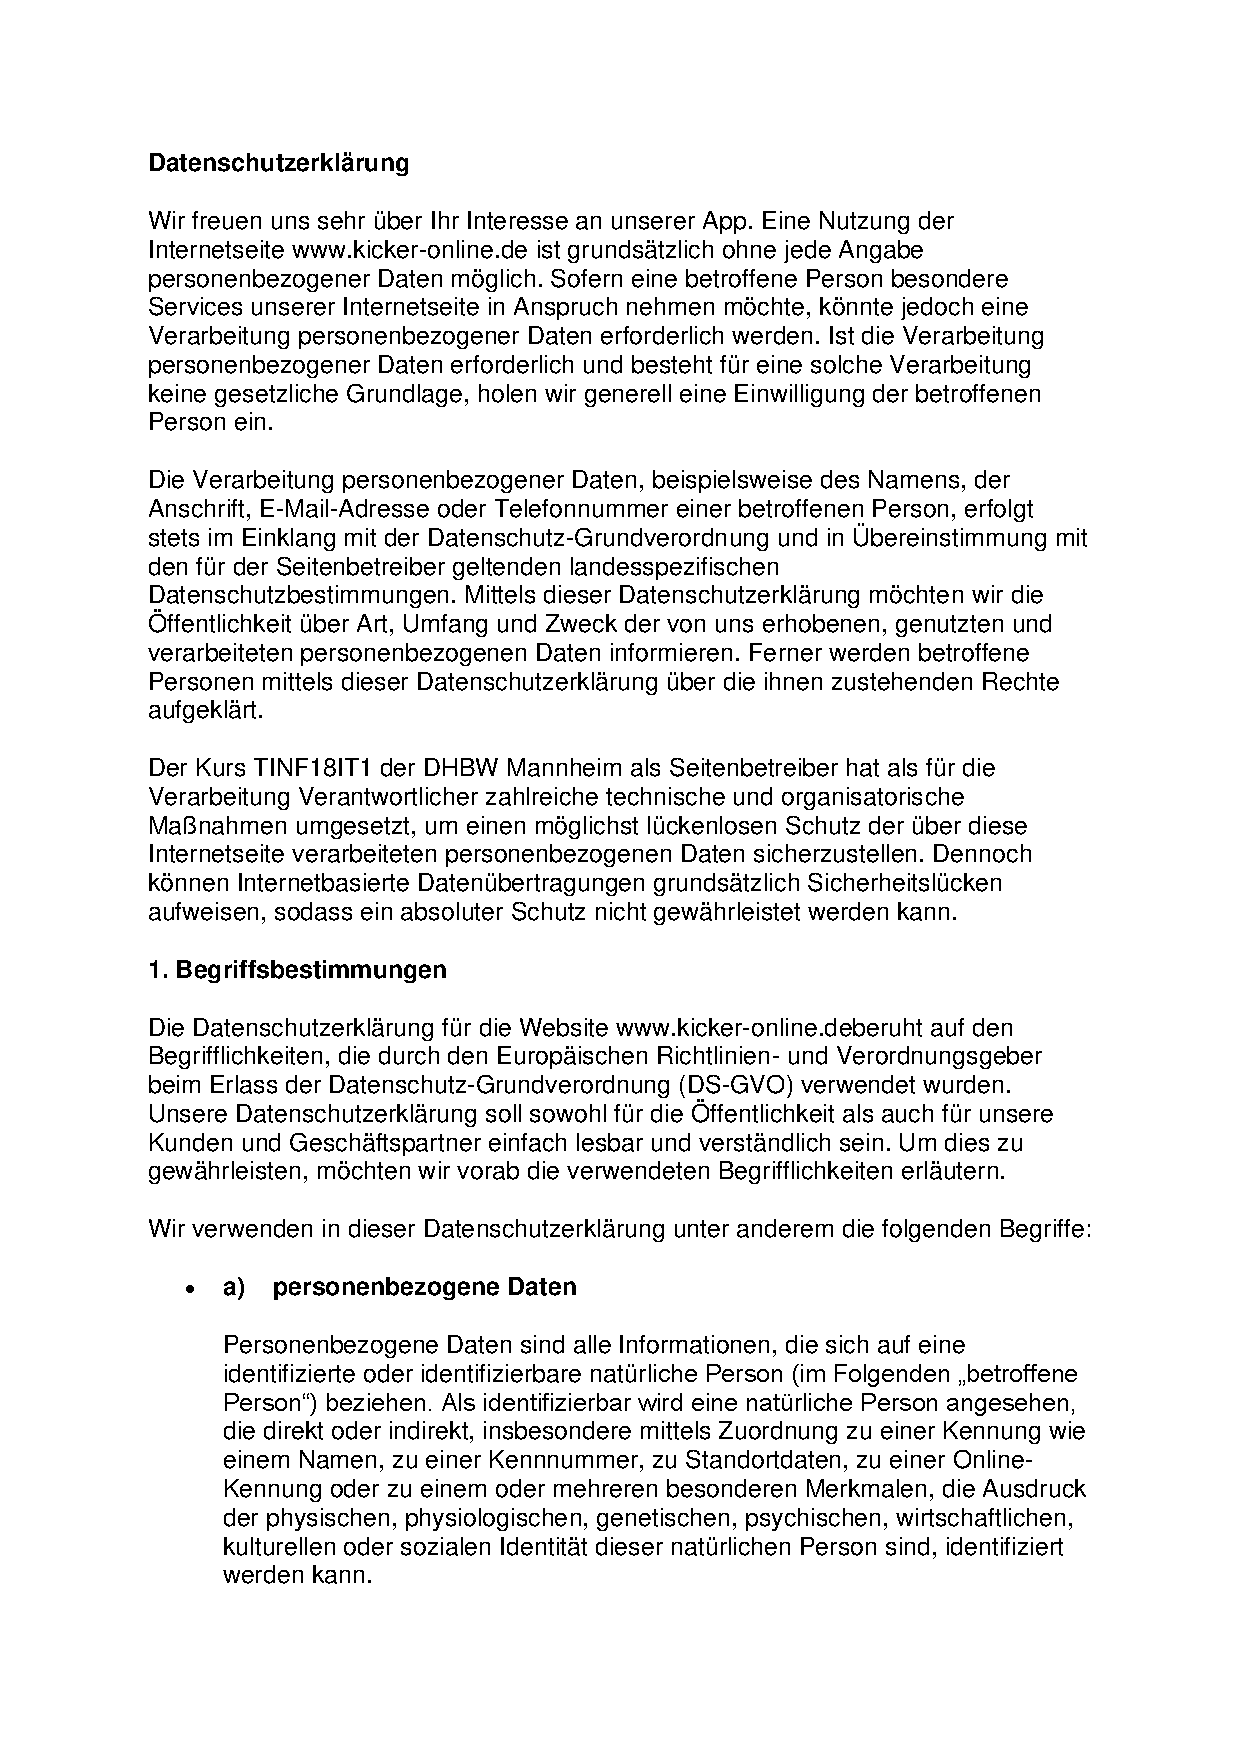
\includepdf[pages={1-}]{../images/text/Datenschutzerklarung}
	
\section*{Impressum}
Das Impressum wurde wie folgt festgelegt:\\\\
\textbf{Impressum}\\
Diese Website wurde im Rahmen der Vorlesung Software Engineering der DHBW Mannheim entwickelt.\\\\
Angaben gemäß §5 TMG\\\\
DHBW Mannheim\\
(Duale Hochschule Baden-Württemberg Mannheim)\\
Coblitzallee 1-9\\
68163 Mannheim\\\\
\textbf{Projektbetreuung}\\
Herr Schultheis\\\\
\textbf{Kontakt}\\
Telefon: +49 621 4105-0\\
E-Mail: info@dhbw-mannheim.de